\uuid{rDGL}
\exo7id{7127}
\titre{exo7 7127}
\auteur{megy}
\organisation{exo7}
\datecreate{2017-02-08}
\isIndication{true}
\isCorrection{true}
\chapitre{Géométrie affine euclidienne}
\sousChapitre{Géométrie affine euclidienne du plan}
\module{Géométrie}
\niveau{L2}
\difficulte{}

\contenu{
\texte{
% angle inscrit, aires
% plus difficile
Une ligne brisée $ABCDE$ formée d'angles de 45 degrés est inscrite dans un cercle. Elle partage le disque en deux régions, chacune d'un côté différent de la ligne. Calculer l'aire de ces deux régions.
% la moitié. 
\begin{center}
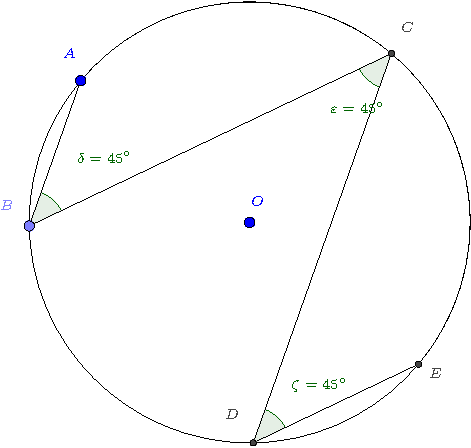
\includegraphics{../images/img007127-1}
\end{center}
}
\indication{Les points $A$ et $E$ sont les extrémités d'un diamètre.  Ensuite, décomposer en triangles.}
\reponse{
Les deux parties ont la même aire.
}
}
